\documentclass[letterpaper,draftclsnofoot,onecolumn,10 pt,compsoc]{IEEEtran} 
\usepackage{graphicx}

%% Language and font encodings
\usepackage[english]{babel}
\usepackage[utf8x]{inputenc}
\usepackage[T1]{fontenc}

%% Sets page size and margins
\usepackage[a4paper,top=1.905cm,bottom=1.905cm,left=1.905cm,right=1.905cm,marginparwidth=1.75cm]{geometry}

%% Useful packages
\usepackage{amsmath}
\usepackage{fancyvrb,cprotect}
\usepackage{graphicx}
\usepackage[colorinlistoftodos]{todonotes}
\usepackage[colorlinks=true, allcolors=black]{hyperref}

%\title{~ \\ ~ \\ ~ \\iCreate: Software Requirements 1.1}
%\author{Hannah Solorzano, Nabeel Shariff, Rhea Mae Edwards \\ ~ \\ Group 61 \\ ~ \\ CS 461, Fall 2017}

\title{
  ~ \\ ~ \\ ~ \\ ~ \\ ~ \\
  Software Requirements 1.1 \\ \bigskip
  \large
  Group 61: iCreate - Generative Design in Virtual Reality \\
  Fall 2017 Term}
\author{Hannah Solorzano - Nabeel Shariff - Rhea Mae Edwards}

\addto\captionsenglish{\renewcommand{\contentsname}{TABLE OF CONTENTS}}

\begin{document}

\maketitle

\vfill

\begin{abstract}
\noindent
%The purpose of this document is to discuss the functionality of the virtual reality program, iCreate, along with covering the general purpose, constraints, terminology, and user characteristics of the program. 
The functionality of the virtual reality program iCreate is described in this document. This document is aimed at specifying requirements of the iCreate software to be developed, along with user characteristics, constraints, and terminology of the program. The product functions, assumptions and dependencies are also detailed within the document. Documentation and a detailed development plan for iCreate are also provided.
\end{abstract}

\newpage

\section*{PARTICIPANTS}
The ICreate - Generative Design in Virtual Reality senior software engineering project consists of the following team members:
\bigskip

\noindent\leavevmode\rlap{}\hfill{\textbf{Raffaele de Amicis,} \textit{Mentor}}\hfill\llap{}\par
\noindent\leavevmode\rlap{Rhea Mae Edwards}\hfill{Nabeel Shariff}\hfill\llap{Hannah Solorzano}\par

\bigskip
\noindent
The following persons are associated with Intel Corporation in regards to Hardware, Software and Development Environments in relations to the project:
\bigskip

\noindent\leavevmode\rlap{}\hfill{\textbf{Mike Premi,} \textit{Co-Mentor}}\hfill\llap{}\par

\bigskip
\noindent
The following persons are guidance mentors as a part of the senior software engineering project course for the students:
\bigskip

\noindent\leavevmode\rlap{\textbf{Kevin McGrath,} \textit{Instructor}}\hfill{\textbf{Behnam Saeedi,} \textit{Teaching Assistant}}\hfill\llap{\textbf{Kirsten Winters,} \textit{Instructor}}\par
\newpage

\tableofcontents

\newpage

\section{INTRODUCTION}
\subsection{Purpose}

The purpose of this user requirements document is to provide a detailed description of the “iCreate” virtual reality (VR) application. This document will illustrate the functions and features of the applications. Additionally, it will explain the interface and system constraints.
\newline

\noindent This document is intended to be proposed to Raffaele de Amicis for its approval and a reference for developing the first version of the system for the development team. 

\subsection{Scope}

The iCreate software is a virtual reality application that allows users to construct complex architectural designs in VR using simple sketches, gestures, and parameters defined by the user. The application will be available to download for systems that can support VR headsets.
\newline

\noindent VR users can provide parameters for a base 3D object that will be used to build the user’s complex design. This objective of modifying the base object, can be done either by manually providing the parameters or by altering the object via gestures or virtual sketches. Moreover, both the base objects and the complex designs can be saved for quick access in the future.
\newline

\noindent Furthermore, the software will need a computer that is capable of running virtual reality applications. The application will also use the proprietary VR software for the respective headset being used.


\subsection{Glossary}

\begin{table}[!hbt]
		% Center the table
		\begin{center}
		% Title of the table
		\caption{Terms and Definitions}
		\label{tab:simParameters}
		% Table itself: here we have two columns which are centered and have lines to the left, right and in the middle: |c|c|
		\begin{tabular}{|c|c|}
			% To create a horizontal line, type \hline
			\hline
			% To end a column type &
			% For a linebreak type \\
			Terms & Definitions\\
            \hline
            VR & Virtual Reality \\
			\hline
			User & Someone who interacts with the iCreate virtual reality application.\\
			\hline
			3D & 3-dimensional\\
			\hline
			Parameters & The measurements for objects defined by the user.\\
			\hline
            Input & Stimulus provided by user.\\
            \hline
            Output & Feedback from the software based on the user’s input.\\
            \hline
            Virtual Space & A 3D area in virtual reality in which the user can move around  and interact with 			  objects.\\
            \hline
            GPU & Graphics processing unit responsible for quick handling and rendering graphics on a 					computer.\\
            \hline
            Generative Design & A form finding process that mimics nature’s evolutionary approach to 					design[2].\\
            \hline
            Render & The process of creating 3D objects and environments.\\
            
            
            % It usually begins  with design goals and then explores innumerable possible permutations of a solution to find the best option.\\
			\hline
		\end{tabular}
		\end{center}
	\end{table}
    
    
\subsection{References}   

[1] IEEE Software Engineering Standards Committee, “IEEE Std 830-1998, IEEE Recommended Practice for Software Requirements Specifications”, October 20, 1998.
\newline

\noindent[2] Autodesk, "Generative Design at Airbus | Customer Stories | Autodesk," Autodesk, [Online]. \\Available: https://www.autodesk.com/customer-stories/airbus. [Accessed 31 October 2017].


\newpage

\section{Overall Description}
\subsection{Product Perspective}
The VR application will utilize a virtual reality headset with input from the user via a controller or gesture recognition software. The VR headset will be used to look around in virtual space while the controllers or gesture recognition software will be used by the user to draw sketches. 
\newline

\noindent The VR application will need to utilize the GPU in a computer to both run the VR application and render 3D objects in the virtual space. Additionally, the 3D modeling will be based on generative design techniques, and the assembly of the complex 3D designs will utilize mathematical equations and algorithms to derive the appropriate structure of the design.

\subsection{Product Functions}
Using the VR application, the user will be able to select and spawn 3D shapes from a provided library and will then be able to adjust the dimensions of the shape. The interface will allow the user to distort or scale the shape to the desired size. Once the shape is finalized, the user sketches a trajectory that represents the curve of the architecture in which they are trying to create. The program will then generate several more of the selected shapes to best fit the curve, forming the structure. If the user wishes, they will be able to store the modified shape and final generated structure in a library for later use.

\subsection{User Characteristics}
There are two main types of users that interact with iCreate: Professional designers and normal users. Each of the types use the system differently, thus, each have their own requirements. 

\begin{itemize}
\item The professional designers will utilize iCreate for professional designs and projects. They will need access to a wide array of curves and precise transformation and design techniques that will enable them to produce state of the art designs.
\item The game designers and students will use iCreate either for entertainment, such as creating simulated environments, or for education, like learning design techniques and concepts.
\end{itemize}

\subsection{Constraints}
%The few constraints that exist for this program pertain to the functions that generate the structure, as well as the hardware that is utilized. For example, when the user creates a 3D shape and trajectory path, if the shape is large in size while the path is small, then the program will not be able to properly generate the structure.
%Secondly, the developers of iCreate, created the program especially to run on the VR hardware, Vivo. Therefore, it would not be possible to run the program on any other types of hardware such as the Oculus. This limits the user base as only those who have the proper VR headset would be able to use this program.

\noindent Firstly, the software constraints for the VR application pertain to the functions that generate complex 3D structures from simple 3D objects. For example, when the user creates a 3D shape and trajectory/path, if the object is larger than the path, or if there are too many objects to fit the path, then the program will not be able to properly generate a complex structure.
\\ \\
\noindent Secondly, the with regards to hardware constraints, the VR application is created specifically for the HTC Vive using the Unity 3D game engine. A VR headset and a computer capable of running VR software are required to use the VR application. As VR programs are graphics intensive,  for iCreate to run successfully, the minimum processor is a Intel Core i5-4590 or AMD FX 8350 (equivalent or better), a NVIDIA GTX 970 or AMD Radeon R9 290 

\subsection{Assumptions and Dependencies}
\begin{itemize}
\item Users have to have enough computing and graphics power to handle VR software and applications.
\item The application must be used with a VR headset.
\item The VR application must allow users to spawn and modify 3D objects.
\end{itemize}


\newpage


\section{Specific Requirements} % Add stretch goals
This section contains all the functional and quality requirements of the system. It gives a detailed description of the system and all its features.

\subsection{External Interface Requirements}

\subsubsection{User Interfaces}
The interface will need to functionally allow the user to spawn a 3D object, then modify it via either a controller or gesture input. Additionally, the user will be able to save to a library for later use or load their creations to create complex structures. Finally, the application will display a way to transform the 3D objects by allowing the user to scale or resize the object.

\subsubsection{Hardware Interfaces}
The VR application will be able to run on a VR headset (preferably a HTC Vive) and a computer that can run VR software.
\\ \\
The minimum CPU and GPU requirements to successfully run the VR application are:
\begin{itemize}
\item Minimum CPU requirements: Intel Core i5-4590 or AMD FX 8350 (equivalent or better)
\item Minimum GPU requirements:  NVIDIA GTX 970 or AMD Radeon R9 290 (equivalent or better)
\end{itemize}

\subsubsection{Software Interfaces}
The VR application will be usable on a Windows operating system capable of running the VR headset’s respective proprietary software.

\subsection{Functional Requirements}
\subsubsection{iCreate VR Environment}
The iCreate software will allow the user to:
\begin{itemize}
\item Move around in VR.
\item Instantiate a simple 3d object.
\item Generate multiple instances of the 3d object.
\end{itemize}

\subsubsection{iCreate Object Library}
The iCreate software will allow the user to:
\begin{itemize}
\item Obtain 3D objects from the application's library.
\end{itemize}

\subsubsection{iCreate Curves}
The iCreate software will allow the user to:
\begin{itemize}
\item To draw a 3D curve.
\item Draw a trajectory in the form of a curve.
\item Create a B-Spline curve.
\item Create a Bezier curve.
\item Create a ellipse curve.
\item Create a circle curve.
\item Create a hyperbola curve.
\item Create a parabola curve.
\item Use the curve to indicate how the user would like to displace multiple instances of the initial object.
\end{itemize}

\subsubsection{iCreate Transformation and Translation}
The iCreate software will allow the user to:
\begin{itemize}
\item Extrude the object.
\item Resize the object.
\item Indicate how they would like to rotate objects across a curve. 
\item Indicate how they would like to translate objects across a curve. 
\item Indicate how they would like to scale objects across a curve. 
\item The 3D objects that make up a complex structure must be connected with each other.
\end{itemize}

\subsubsection{iCreate Save and Load}
The iCreate software will allow the user to:
\begin{itemize}
\item Import geometry from a .fbx extension file format.
\item Import a 3D object.
\item Save a 3D object.
\item Save structures.
\item Save the entirety of the project as a whole.
\end{itemize}

\subsubsection{iCreate Stretch Goals}
After the completion of the iCreate program, the developers plan to use a robot to take the design created in the VR space, and recreate it in real life. 
\begin{itemize}
\item The robot will be provided by the Oregon State University Robotics Club.
\item An application programming interface (API) library will be used to allow the robot to read and apply the design.
\end{itemize}

%\begin{itemize}
%\item The system shall allow the user to use controllers or gestures as input.
%\item The system shall allow the user to spawn 3D objects through the input as output.
%\item The system shall allow the user to move around the virtual 3D environment.
%\end{itemize}

\subsection{Performance Requirements}
The iCreate program should be able to run on a computer with at least an Intel Core i5-4590 or AMD FX 8350 (equivalent or better), a NVIDIA GTX 970 or AMD Radeon R9 290 (equivalent or better) graphics card, at least 4GB of RAM, at at least 30 frames per second. 
\\ \\
The requirements to run iCreate will also depend on the user and the scale or intricacy of the architectural structure that is designed as a larger, more complex structure will require more processing power and a stronger graphics card.

\subsection{Design Constraints}
The VR program will have to run on a HTC Vive VR headset, and be able to support both controller and gesture input through Leap Motion and Lighthouse Tracking Technology. The user interface must be able to allow the user to spawn and transform 3D objects, and save and load previous creations.

\subsection{Gantt Chart}
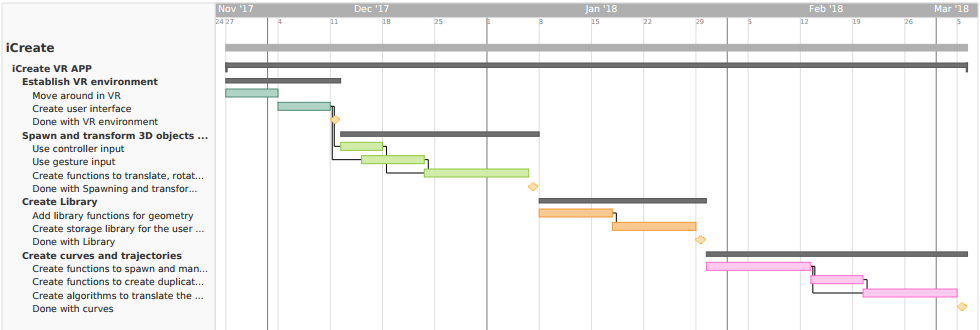
\includegraphics[width=\textwidth]{Gantt_chart2.PNG}
\end{document}